%# -*- coding: utf-8-unix -*-
%%==================================================
%% chapter04.tex for SJTU Bachelor Thesis
%%==================================================

%\bibliographystyle{sjtu2}%[此处用于每章都生产参考文献]
\chapter{基于深度增强学习的流量优化系统}
\label{chap:System}
基于前文对于增强学习算法、数据中心的流量特点、负载均衡算法及流量调度问题的讨论,我们提出一种可以根据5G Cloud RAN架构下的数据中心网络流量实时动态地调整参数以达到最优负载均衡的系统——基于深度增强学习的流量优化系统。该系统解决了数据流在数据链路上从端系统、边缘交换机\footnote{在数据中心网络结构中叶结点交换机、边缘交换机、架上(Top of Rack,简称为ToR)交换机均指与端系统直接相连的交换机,聚合交换机(aggregation switches或aggregate switches)和核心交换机(core switches)相当于叶脊结构中的脊结点交换机(spine switches)}、聚合交换机、核心交换机直到目的地址的传输过程中历经的发送、入队、拥塞信息采集、选路等问题,将使用增强学习的流量调度算法和负载均衡机制相结合,给出数据中心网络中流量优化的一种解决方案。与Li Chen等人的工作\cite{chen2018auto}不同,本文更关注于负载均衡机制效果的优化。

\section{系统架构}
本文提出的系统采用混合型结构,由集中式的流量调度算法和分布式的负载均衡机制两部分组成。集中式流量调度是一种基于PIAS架构的多层次调度机制,MLFQ所采用的阈值参数和大数据流均由核心层设置和处理,核心层负责向外围层分发MLFQ队列的阈值、周期性采集数据流量信息等,端系统与交换机之间的通信采用包含ECN通知的legacy TCP协议。负载均衡机制采用DRILL分布式均衡算法,利用网络虚拟化技术中的封装格式实现拥塞信息的采集工作,以维护选路用的拥塞信息表。

\begin{figure}[ht]
\centering
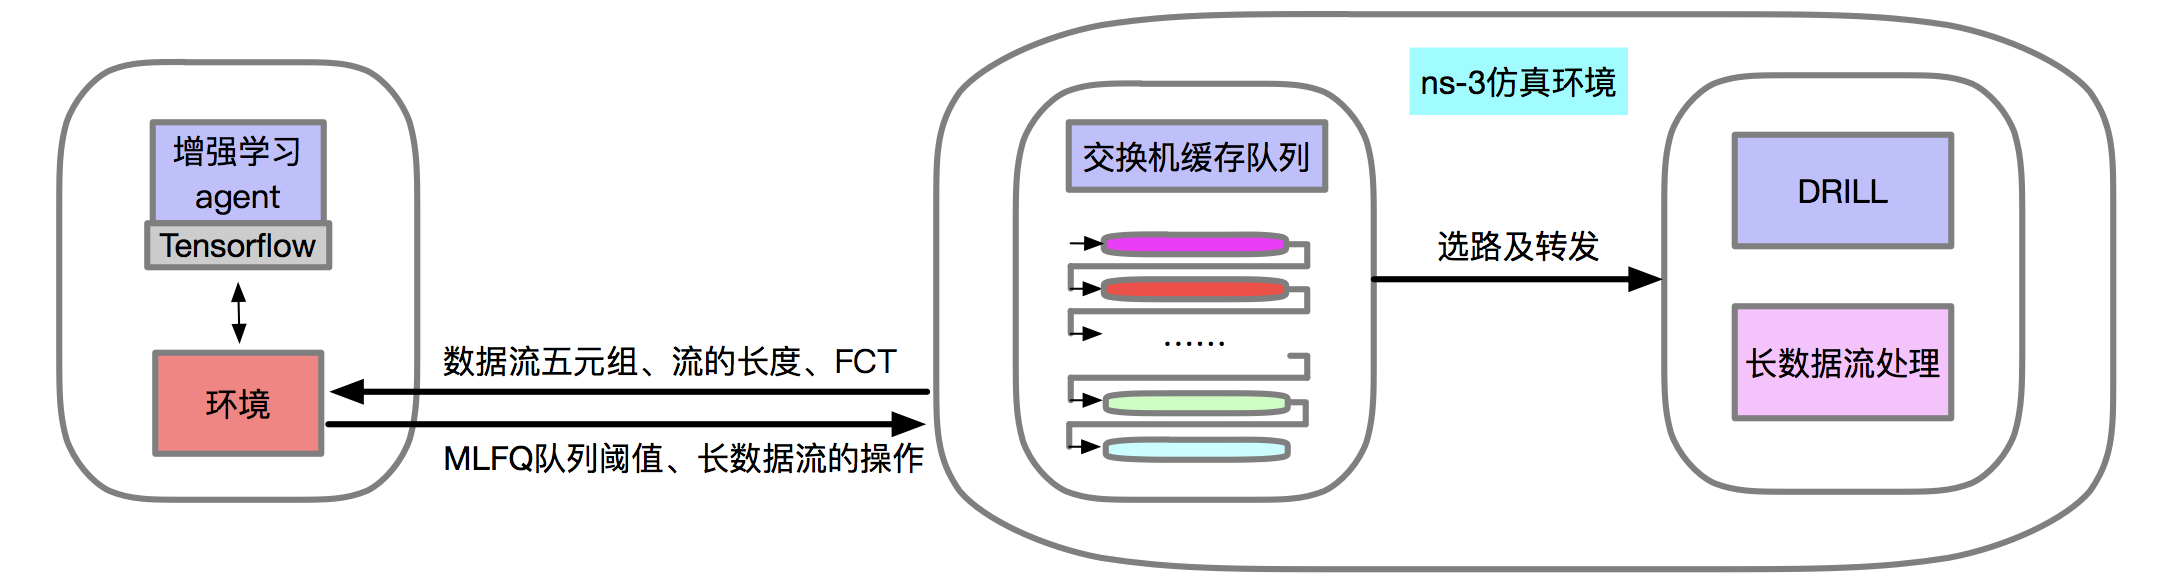
\includegraphics[width=16cm]{figure/architecture.png}
\caption{系统整体架构}
\label{fig:architecture}
\end{figure}
\subsection{集中式流量调度}
目前将深度增强学习算法应用于数据中心网络的主要问题是数据流信息采集与决策生成之间的较长延迟,对于当前数据中心大于10Gbps的链路带宽,要想达到数据流级别的优化,操作的往返延迟至少要在毫秒级,如果不引入特殊设计的硬件这对于深度增强学习是不可实现的。鉴于数据中心网络数据流大小的长尾分布,应该把短数据流的处理在端系统处解决,将较长的数据流交给一个中心组件处理。PIAS架构利用MLFQ解决流量调度这一问题,刚好适合于深度增强学习算法,这是因为MLFQ的降级阈值需要靠计算确定,以适应特定环境。另外,当较长的数据流被降级到某优先级后,就可以交由中心组建处理,对长数据流的路由、速率限制、优先级等做出单独的决策,而这一过程同样可由深度增强学习算法来实现。
\subsubsection{MLFQ阈值的确定}
PIAS采用分布式的数据包标记,在每个端系统处有$k$个优先级$P_i$,$1 \leq i \leq K$和$(K-1)$个降级阈值$\alpha_j$,$1 \leq j \leq K-1$,其中从$P_1$到$P_K$的优先级依次递减,$\alpha_1 < \alpha_2 < … < \alpha_{K-1}$。每当端系统生成一个新的数据流,它的数据报文会被标记为最高优先级,随着其发送的字节数越来越多,该数据流的数据包优先级逐渐下降到$P_j (2 \leq j \leq K)$。从$P_{j-1}$降级到$P_j$的阈值是$\alpha_{j-1}$。我们假定$\alpha_K$为正无穷,这样最大的一些数据流的后发送的数据包都在第K个优先级的队列中。标记利用的是IP报文的DSCP域。通过数据流的已发送字节数和降级阈值,端系统可以做本地化的决定。当网络流量情况变化时,由中心组件对队列的降级阈值做调整。
我们定义数据流大小的累积分布函数$F(x)$\footnote{$F(x)$:任一给定数据流的大小比x字节小的概率},并用$L_i$表示给定数据流带给第$i$级队列$Q_i$($i = 1, ..., K$)的数据包的个数。由优先级队列的定义可知,$L_i$的期望:$E[L_i] \leq (\alpha_i - \alpha_{i-1})(1-F(\alpha_{i-1}))$。定义数据流的到达速率为$\lambda$,那么数据包到达第$i$级队列$Q_i$的速率$\lambda_i = \lambda E[L_i]$。队列的服务速率取决于更高优先级的队列是否为空,因此当链路的服务速率为$\mu$时,最高优先级$P_1$的容量总为$\mu_1 = \mu$。定义$\rho_i = \lambda_i / \mu_i$为$Q_i$的利用率,则$Q_1$的空闲率为$(1-\rho_1)$,$Q_2$的服务速率为$\mu_2 = (1-\rho_1)\mu$。依此类推,我们有$\mu_i = \prod_{j=0}^{i-1} (1-\rho_j) \mu, \rho_0 = 0$。队列i的平均延迟时间$T_i = 1/(\mu_i - \lambda_i)$。对于一个大小在$[\alpha_{i-1},\alpha_i)$区间内的数据流,它将经历不同优先级队列造成的延迟直到它到达第i级队列。令$i_{max}(x)$为比$x$大的最小阈值队列级数,那么对于大小为$x$的数据流,其平均FCT:$T(x) \leq \sum_{i=1}^{i_{max}(x)}T_i$。我们用$g_i = F(\alpha_i)-F(\alpha_{i-1})$表示大小落在$[\alpha_{i-1},\alpha_i)$区间内的数据流的百分比,因此,$g_i$就是两个连续队列阈值之间的间隔。如果用$g_i$等价地表示$\alpha_i$($g_i \geq 0, i = 1, ..., K-1$),FCT最小化问题就可以表达为如下形式:
\begin{equation}
\label{eq:target}
%\begin{align}
    \min_{\text{g}} \tau(\text{g}) = \sum_{l=1}^{K}(g_l \sum_{m=1}^{l}T_m) = \sum_{l=1}^K(T_l \sum_{m=l}^K g_m) 
%\end{align}
\end{equation}

我们将上式转换成增强学习的语言:
\begin{itemize}
    \item 状态空间:状态由网络中当前时刻t已完成数据流的集合$F_t^d$表示。每个数据流由一个5元组确定:源/目的IP地址,源/目的端口号,传输协议。由于这里只考虑已完成的数据流,数据流的FCT和大小被看作是流的属性,即一个数据流共有7个特征。
    \item 动作空间:动作空间由中心组件计算得到,在时间t,由agent确定的动作(或决策)是一组MLFQ的队列阈值${\alpha_i^t}$。
    \item 奖励:环境给agent反馈的奖励是对前一时刻的动作有多好的评价,这里将连续两个时刻的目标函数的比值作为奖励:$r_t = \tau_{t-1} / \tau_{t}$。它标志着前一时刻的动作是否导致了FCT的降低,或者对于整体性能有所提升。
\end{itemize}

由于此增强学习问题的动作空间是连续的,应采用第\ref{sec:DPG}小节中的DPG算法。如算法\ref{dpgalgo}所示,对于某时刻从端系统新到达的数据流采用深度神经网络进行学习,在经验回放机制中存储一个四元组${s_t, a_t, r_t, a_{t+1}}$。奖励(或称回报)$r_t$和下一时刻的状态$s_{t+1}$是在端系统的下一次更新时获得的,因此agent需要在缓存中保留$s_t$和$a_t$直到收集完四元组的所有元素。神经网络的参数更新是从经验回放机制的记忆库中随机选取一批特定数量的四元组,以实现更稳定的学习过程、避免参数不收敛。通过计算前后时刻的目标函数的商,可以得到后一时刻的动作的奖励,运用actor-critic算法最终实现式\ref{eq:target}的解决(网络结构如图\ref{fig:ddpg_tensor})。
\begin{figure}[ht]
\centering
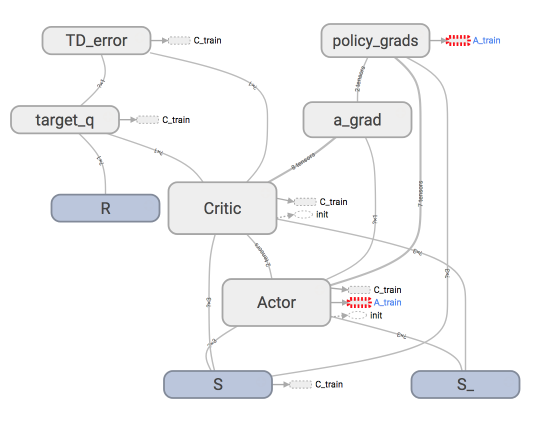
\includegraphics[height=6cm]{figure/DDPG.png}
\caption{DDPG网络模型在tensorboard中的结构图}
\label{fig:ddpg_tensor}
\end{figure}
\subsubsection{长数据流的处理}
我们将MLFQ的最后一个阈值$\alpha_{K-1}$作为判断长数据流和短数据流的标准,大于该值的数据流均由本地处理。作为上述DDPG算法的输出值,$\alpha_{K-1}$是根据网络情况实时变化的。对于长数据流,我们同样采用PG算法:
\begin{itemize}
    \item 状态空间:状态由当前时刻t网络中所有活跃的数据流$F_t^a$和已完成数据流的集合$F_t^d$表示。每个数据流由5元组确定,除此之外活跃数据流还有一个优先级的属性;已完成的数据流有流的大小和FCT属性。
    \item 动作空间:对于t时刻的每一个数据流f,agent为它做出的动作是${Q_{t}(f), R_{t}(f), P_{t}(f)}$,其中$Q_{t}(f)$是数据流的优先级,$R_{t}(f)$是速率限制,$P_{t}(f)$是数据流的传输路径。$Q_{t}(f)$是从数据流到优先级的映射,即$Q_{t}(f) \in [1,K]$。
    \item 奖励:只计算已完成数据流的回报:可以选择发送速率、链路利用率、连续时刻的吞吐量的比值或差等。由于较难实时获取数据流级别的信息,这里选择对于已完成数据流的前后时刻平均吞吐量的比值作为回报。
\end{itemize}
考虑到DDPG的收敛相对较慢,以及状态空间可以表达为一个离散空间,此处对于长数据流的处理采用Stochastic策略梯度方法(详见第\ref{sec:stochas_PG}小节)。网络结构如图\ref{fig:stochas_pg}所示。
\begin{figure}[ht]
\centering
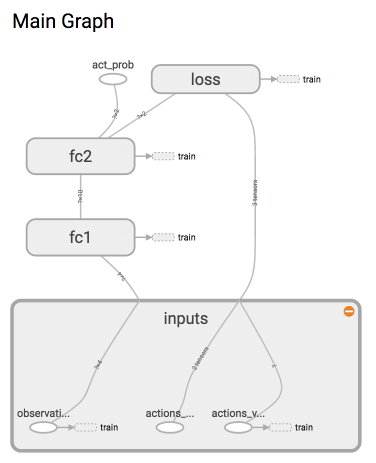
\includegraphics[height=7cm]{figure/dpg.png}
\caption{Stochastic策略梯度方法的神经网络在tensorboard中的结构图}
\label{fig:stochas_pg}
\end{figure}
%\subsubsection{交换机的部署}
%系统中的交换机的设置需要满足两个条件:优先级调度(使用MLFQ队列)和允许ECN标记(当交换机的缓存占用率高于标记阈值时,新到达的数据包就被标记为经历过拥塞)。
%\subsubsection{速率控制}

\subsection{分布式负载均衡}
本小节的负载均衡是针对短数据流而言的,这是因为当长数据流在端系统处的已发送字节大于一定阈值后,它们的数据报文会被降级至较低优先级队列交由中心组建处理。如前面讨论过的,由于深度增强学习的运行时间不允许对于每一个数据流实时做出决策,因此我们在短数据流的负载均衡机制中采用分布式的方法,即不由中心组件控制选路等过程。我们在第\ref{sec:loadBalance}小节中讨论的负载均衡算法选出一种适合于本文环境的算法。首先,MPTCP算法主要基于ECMP路由机制,当其中的子流被分配至一条拥塞情况较严重的路径时,对于其性能的影响较大,且使用多条链路有时只能带来有限的增益;作为负载均衡问题的经典算法CONGA,尽管其仿真结果上表现很好,但由于它需要对交换机的软件进行修改,并采用VxLAN的头部传输链路拥塞信息,这对于大型数据中心网络的部署和实际效果有一定影响(等待拥塞信息的反馈常常需要花费几个往返时延);与CONGA算法相似,CLOVE也采用了虚拟化技术,需要对交换机软件进行修改;Expeditus的拥塞信息采集的延迟对于实际场景中也较长,且其对于网络拓扑有较严格要求,不是一种较为普适的模型;和MPTCP一致,Presto也是基于ECMP均衡机制,由于ECMP在实际部署时可能存在重大问题,且Presto的数据流分割对于PIAS架构是不适用的;LocalFlow在面对拥塞情况时可能表现很差,其调度的间隔较长,不能保证对于拥塞情况的实时处理;而DRILL负载均衡机制不仅满足了我们对于短数据流实时性处理的要求,且其不需要更改硬件或协议等,在不同场景下表现均很好,我们在分布式负载均衡中选择DRILL算法。
\subsection{网络拓扑}
仿真所用的网络拓扑采用如图\ref{fig:netw_archi}所示的叶脊结构:一台核心交换机下连有六台聚合交换机,每两个聚合交换机组成一个pod,一个pod中有三台叶结点交换机,叶结点交换机直接与端系统相连。
\begin{figure}[ht]
\centering
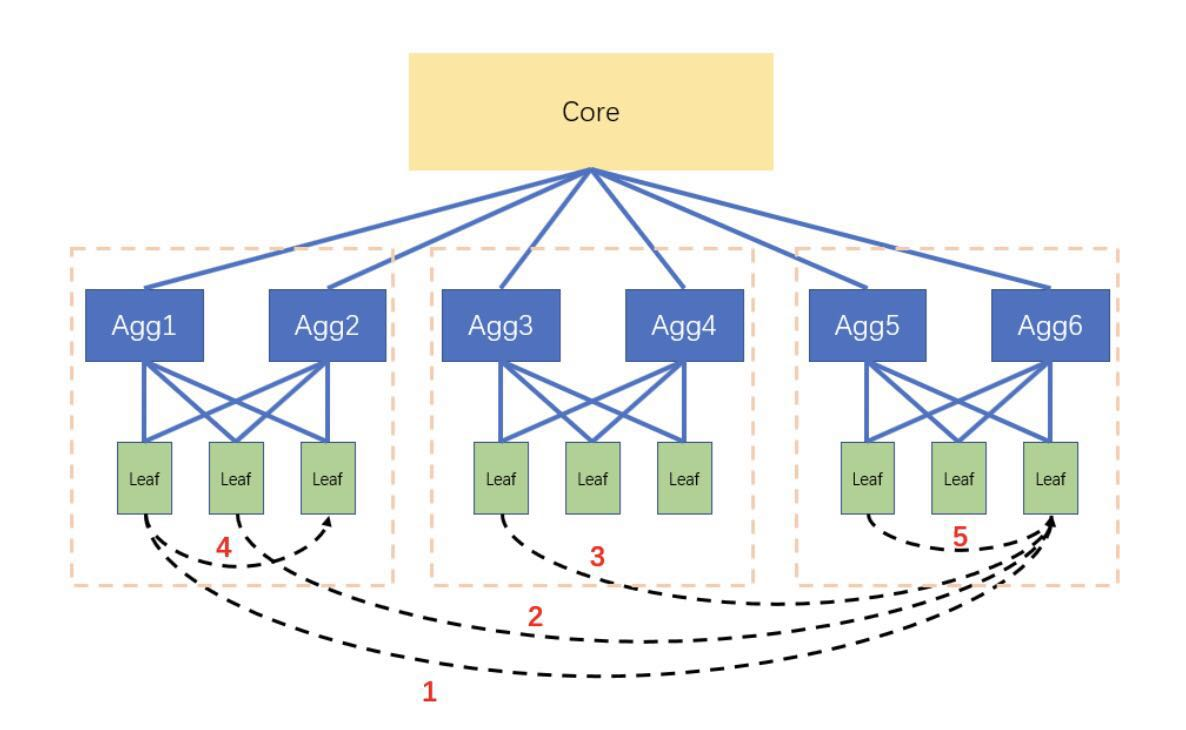
\includegraphics[height=5cm]{figure/topo.jpeg}
\caption{仿真所用的网络拓扑}
\label{fig:netw_archi}
\end{figure}



\section{仿真过程}
为了检测本文提出的流量优化系统的性能效果,我们对比了ECMP、CONGA、DRILL和本文的模型在ns-3仿真环境下的FCT、总传输时延和平均链路利用率。系统中的中心组建深度增强学习模型是用TensorFlow深度学习框架\cite{tensorflow}实现的,通过在具有两块NVIDIA GeForce GTX 1080 Ti显卡的服务器\footnote{Intel Xeon CPU E5-4640 v3 @ 1.90GHz,48 CPUs,Ubuntu 17.10,GNU/Linux 4.13.0-21-generic x86\_64}上预训练,使得神经网络的参数不断收敛,学习到不同模式、不同数据流下的最优MLFQ参数与长数据流的调度方法。
\subsection{仿真环境搭建}
笔者在服务器上安装了Docker平台\cite{docker},在容器(container)中运行仿真环境ns-3。由于增强学习算法需要利用GPU,且Docker中已有增强学习模块的镜像(image),因此我们采用编译dockerfile的方式构建自己的镜像(如图\ref{fig:merge}所示),再从该镜像实例化为容器。由于我们希望能够看到增强学习的训练过程,我们在容器中额外开放一个端口使它能运行jupyter notebook服务\footnote{从镜像实例化容器的命令行为“sudo nvidia-docker run -d -p 7771:8888 why2011btv/ns-3.rl-gym”,进入该容器的命令行为“docker exec -it 510fb70d5fc4 bash”。}。我们利用ns-3中提供的Ethernet Switch和Standard Host模块实现常规以太网交换机和端系统,在github中snowzjx/ns3-load-balance repository\footnote{https://github.com/snowzjx/ns3-load-balance}的基础上实现ECMP、CONGA、DRILL以及本文提出的架构的仿真。

\begin{figure}[ht]
\centering
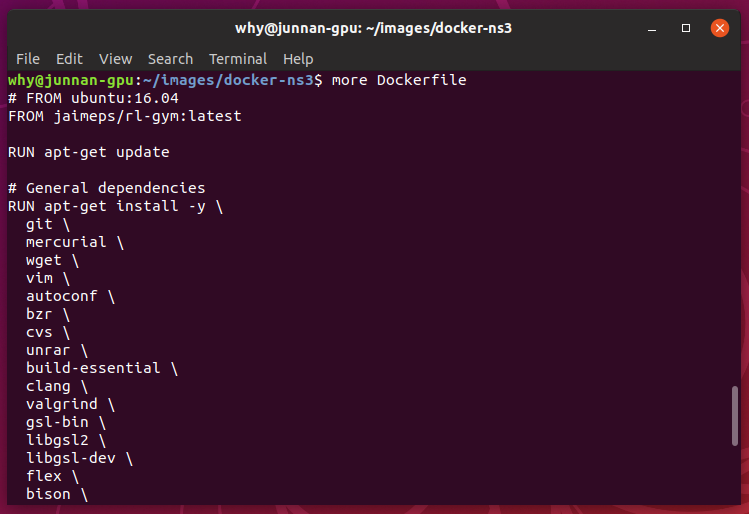
\includegraphics[height=5cm]{figure/merge.png}
\caption{从dockerfile构建自己的镜像,其中``From jaimeps/rl-gym:latest"这一行显示了本仿真环境的基础镜像rl-gym,后续行均为在其基础上构建ns-3环境的过程}
\label{fig:merge}
\end{figure}

\begin{figure}[ht]
\centering
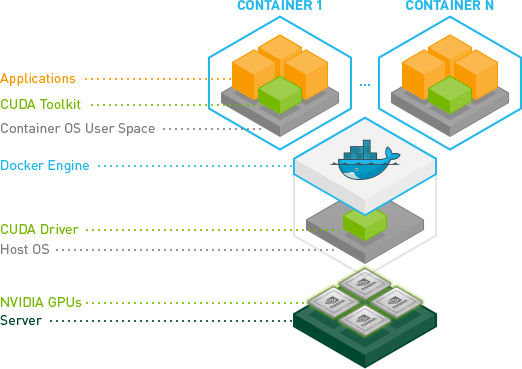
\includegraphics[height=5cm]{figure/docker.png}
\caption{Docker平台与容器}
\label{fig:docker}
\end{figure}



\subsection{增强学习深度模型的训练}

深度增强学习算法主要涉及两个模型的训练,一个是为确定MLFQ队列阈值的DDPG,一个是长数据流处理的Stochastic Policy Gradient。其中,DDPG用到了两个全连接的隐藏层,分别有600个神经元,输出层共$K-1$个神经元,对应$K-1$个队列阈值。输入层接收状态输入,由700个神经元表示。Stochastic PG神经网络由10层全连接的隐藏层表示,每层有300个神经元,agent接收的状态信息由700个神经元作为输入层。二者均训练约8小时,参数的收敛与否可以从系统得到的reward上判断(如图\ref{fig:cognitive})。训练过程中,数据流的FCT与训练时长如图\ref{fig:trainingprocess}所示,可以看到训练过程反映在FCT上是较平稳的。


\begin{figure*}[htb!]
\centering
\begin{subfigure}{0.47\textwidth}
     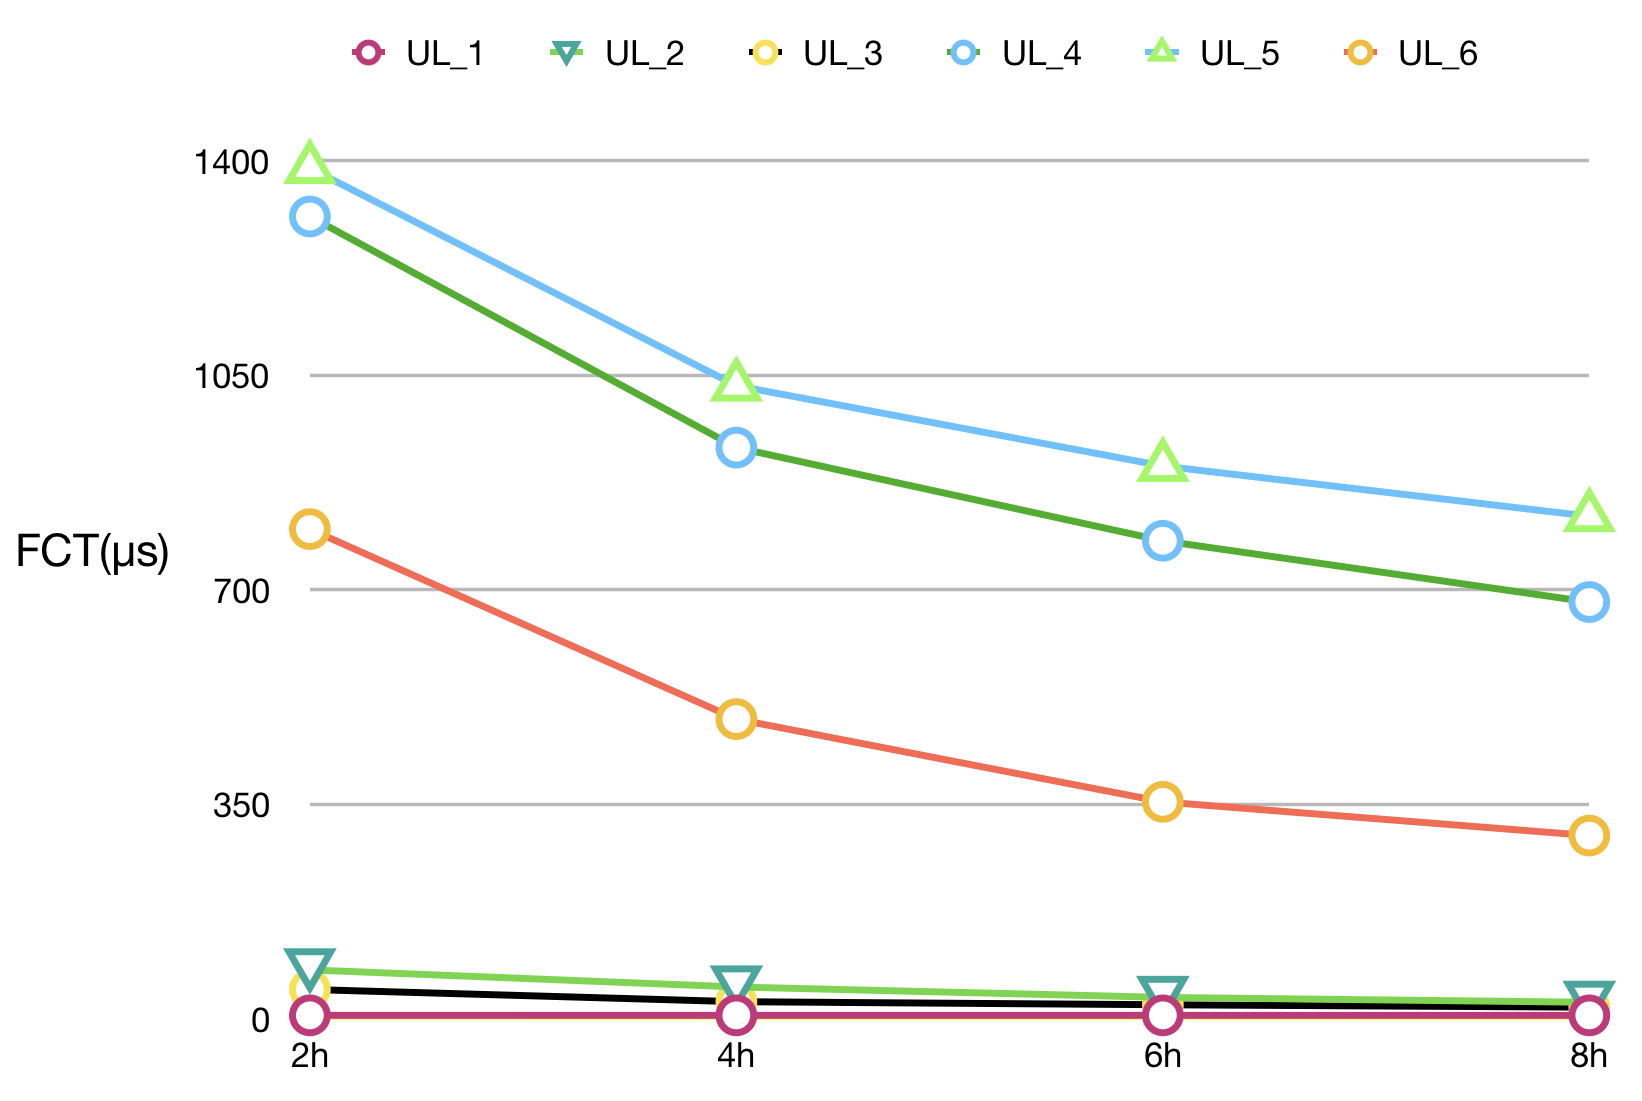
\includegraphics[width=\textwidth]{figure/train_8h.png}
     \caption{训练过程中pod内数据流FCT的变化曲线}
\end{subfigure}\hspace{2em}
\begin{subfigure}{0.47\textwidth}
%\centering
    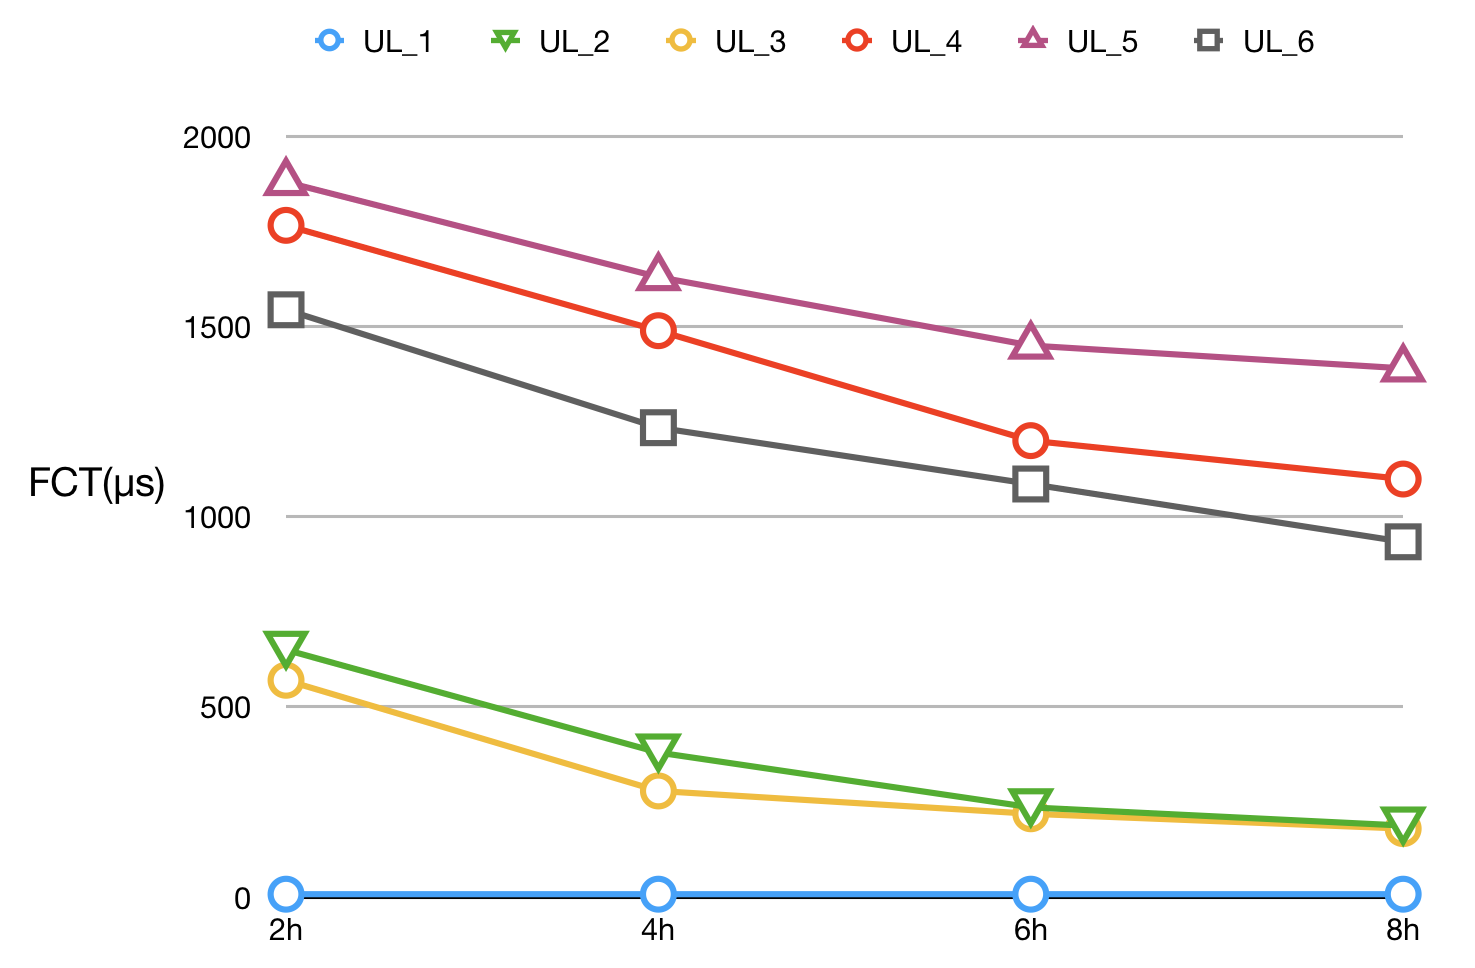
\includegraphics[width=\textwidth]{figure/train_8h1.png}
     \caption{训练过程中pod间数据流FCT的变化曲线}
\end{subfigure}%\hspace{0.277em}
\caption{FCT与训练时长折线图}
\label{fig:trainingprocess}
\end{figure*}

\begin{figure}[ht]
\centering
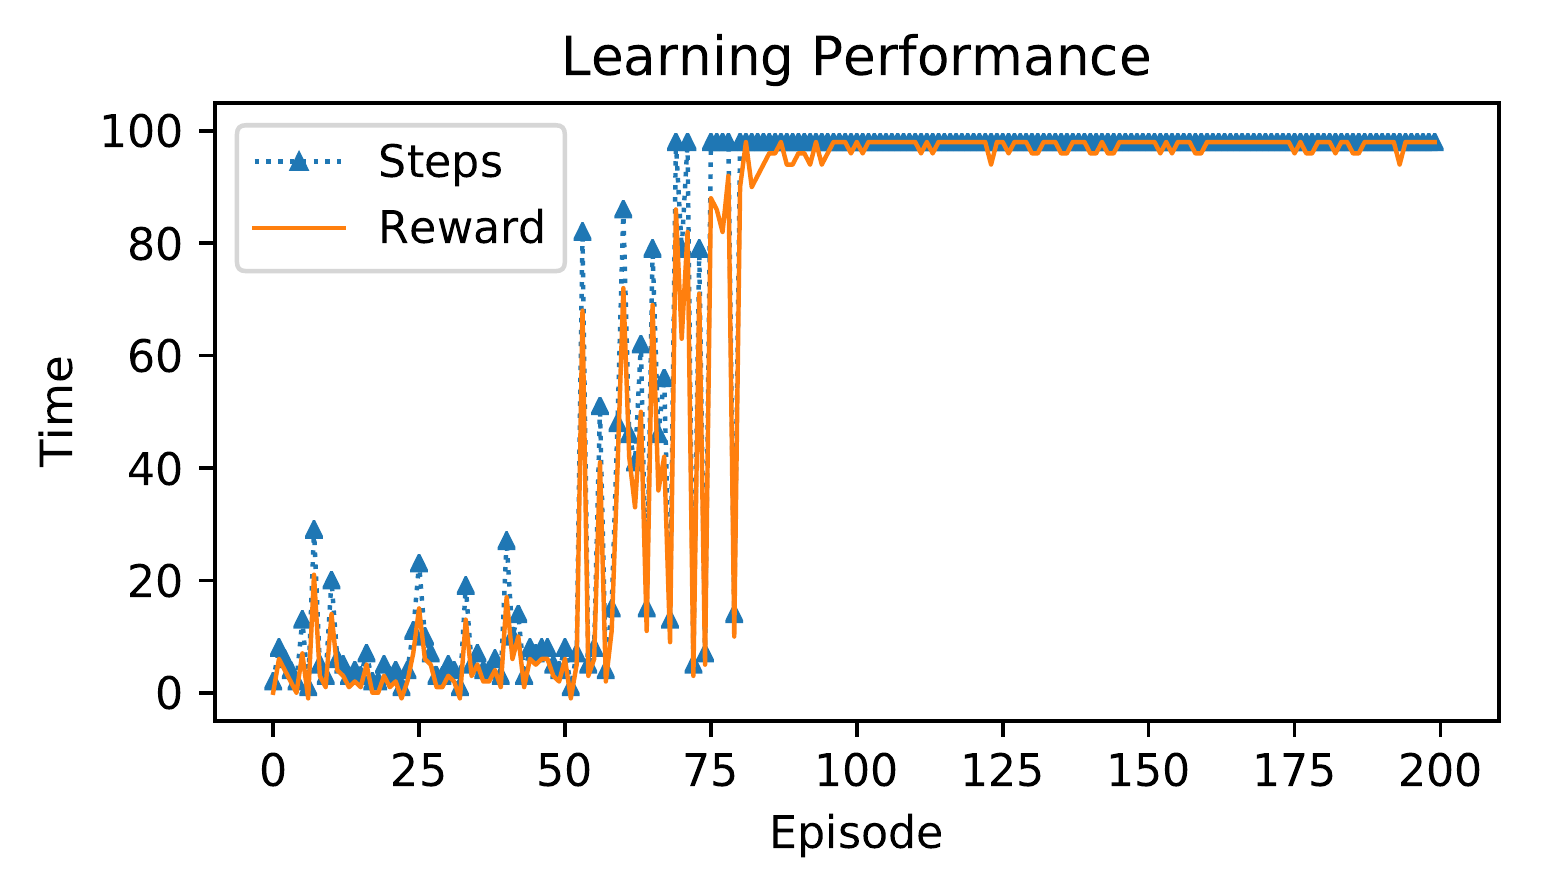
\includegraphics[height=6cm]{figure/cognitive-learning.png}
\caption{Stochastic Policy Gradient训练过程}
\label{fig:cognitive}
\end{figure}
\subsection{仿真数据源}
仿真所用的数据源如图\ref{fig:datasource}所示。
\begin{figure}[ht]
\centering
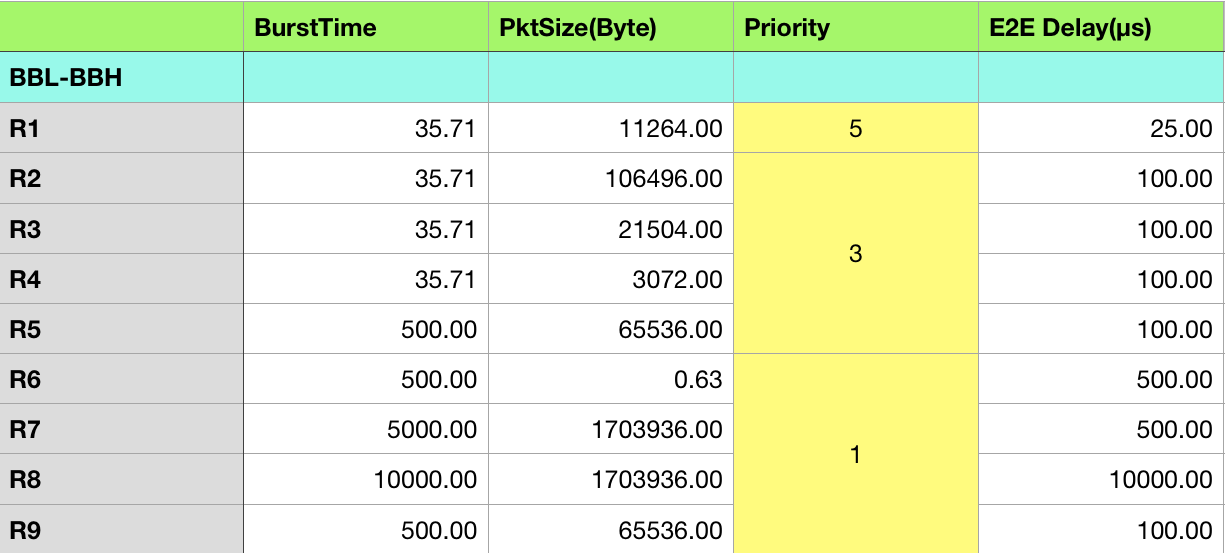
\includegraphics[height=4cm]{figure/source.png}
\caption{仿真数据源}
\label{fig:datasource}
\end{figure}

\subsection{仿真结果}
\subsubsection{流完成时间}
从图\ref{fig:podfct}可以看出,MLFQ将数据流分为两批进行处理,短数据流使用DRILL算法,长数据流由中心组件单独处理,均可以达到比之前的算法(ECMP、CONGA、DRILL)更好的性能,当然由于系统主要利用DRILL算法进行负载均衡,因此在部分数据流的表现上与DRILL相近。考虑到数据中心网络的数据流符合长尾分布的特征,对于长数据流的处理是至关重要的,本文的系统在长数据流上的表现是所有参考算法中最好的(pod内带来至少8.9\%的FCT提升、pod间带来至少7.4\%的FCT提升)。另外,对于流量负载较轻的网络,几种算法的表现的差别不大;当流量负载增加时,可以看到本文提出的系统对FCT有较明显的提升。

\begin{figure*}[htb!]
\centering
\begin{subfigure}{0.47\textwidth}
     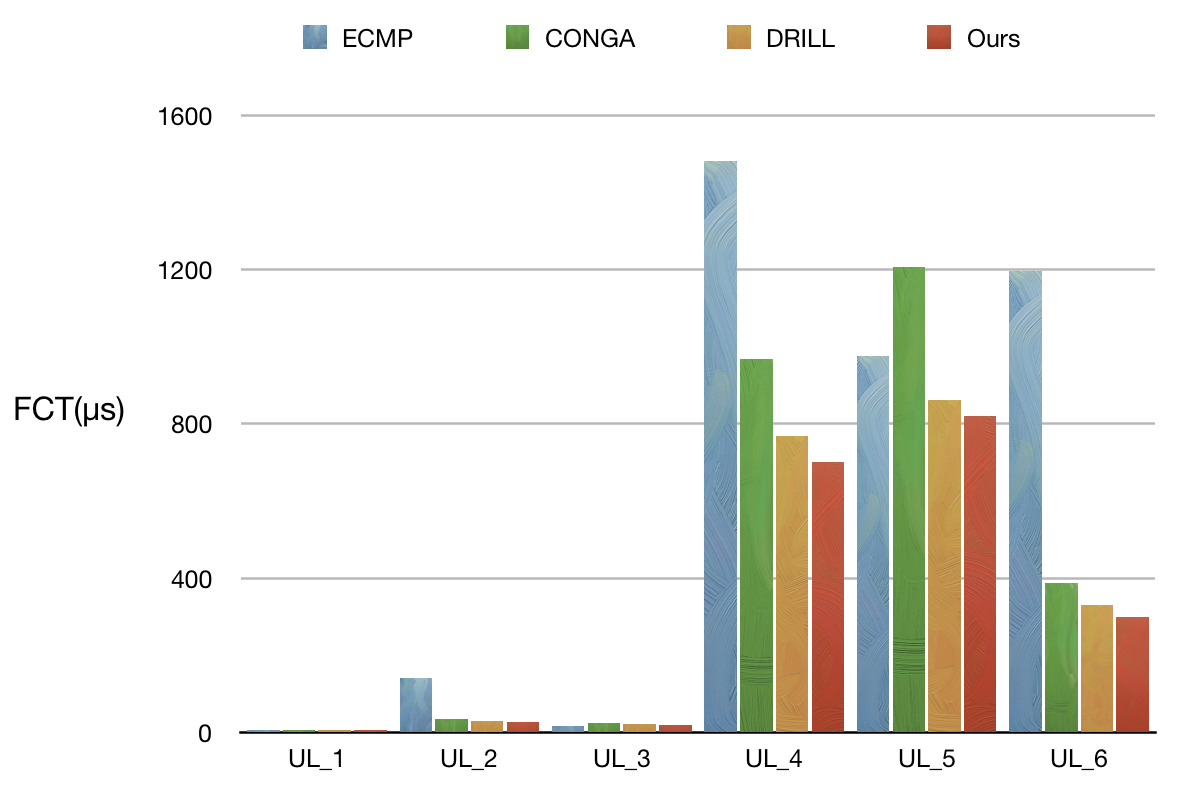
\includegraphics[width=\textwidth]{figure/intrapod.png}
     \caption{pod内不同数据流的FCT}
\end{subfigure}\hspace{2em}
\begin{subfigure}{0.47\textwidth}
%\centering
    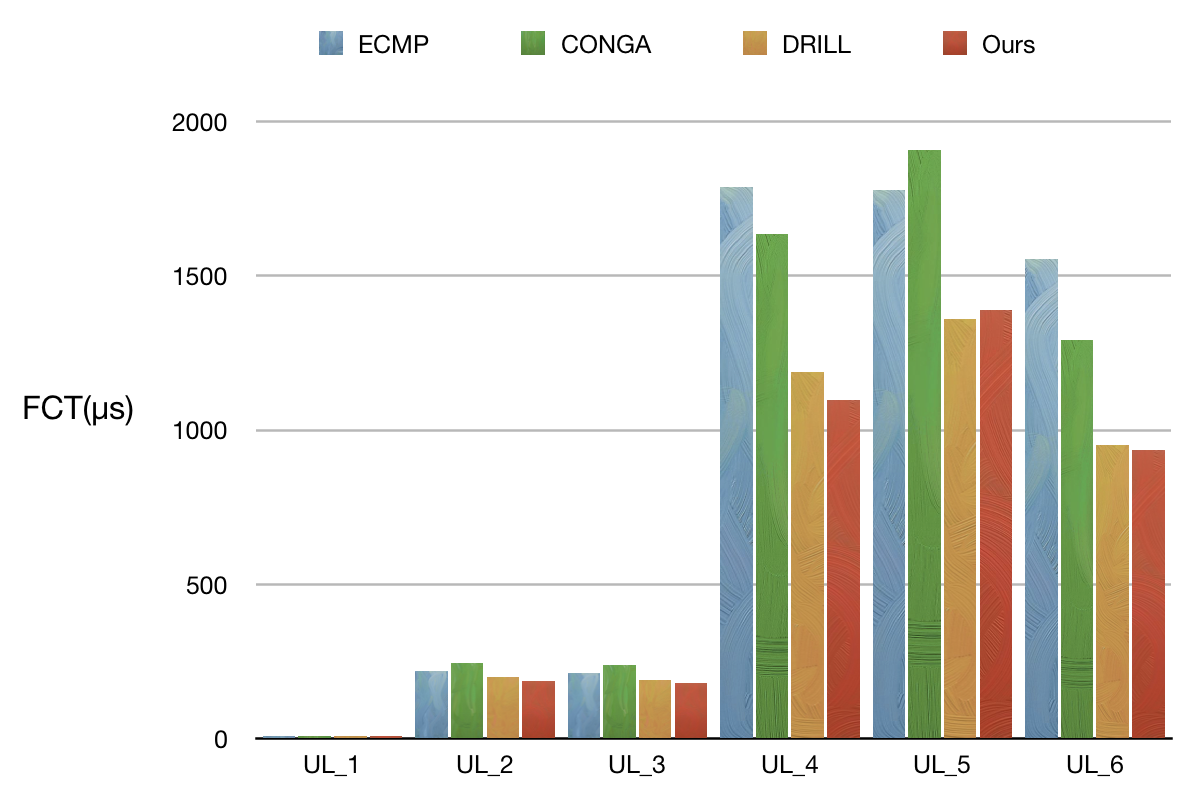
\includegraphics[width=\textwidth]{figure/interpod.png}
    \caption{pod间不同数据流的FCT}

\end{subfigure}%\hspace{0.277em}
\caption{数据流完成时间}
\label{fig:podfct}
\end{figure*}


\subsubsection{总传输时延}
通过测量数据发往不同pod的端口(本组实验共设置5个端口)可以比较选路过程上各个算法的优劣。总体而言,CONGA与ECMP的完成时间相近,DRILL和本文的系统相近,在涉及不同pod间的数据传输(路径需要经过聚合交换机)和平均完成时间较长的数据,本文系统均表现优异,结果如图\ref{fig:total_time}所示。
\begin{figure}[ht]
\centering
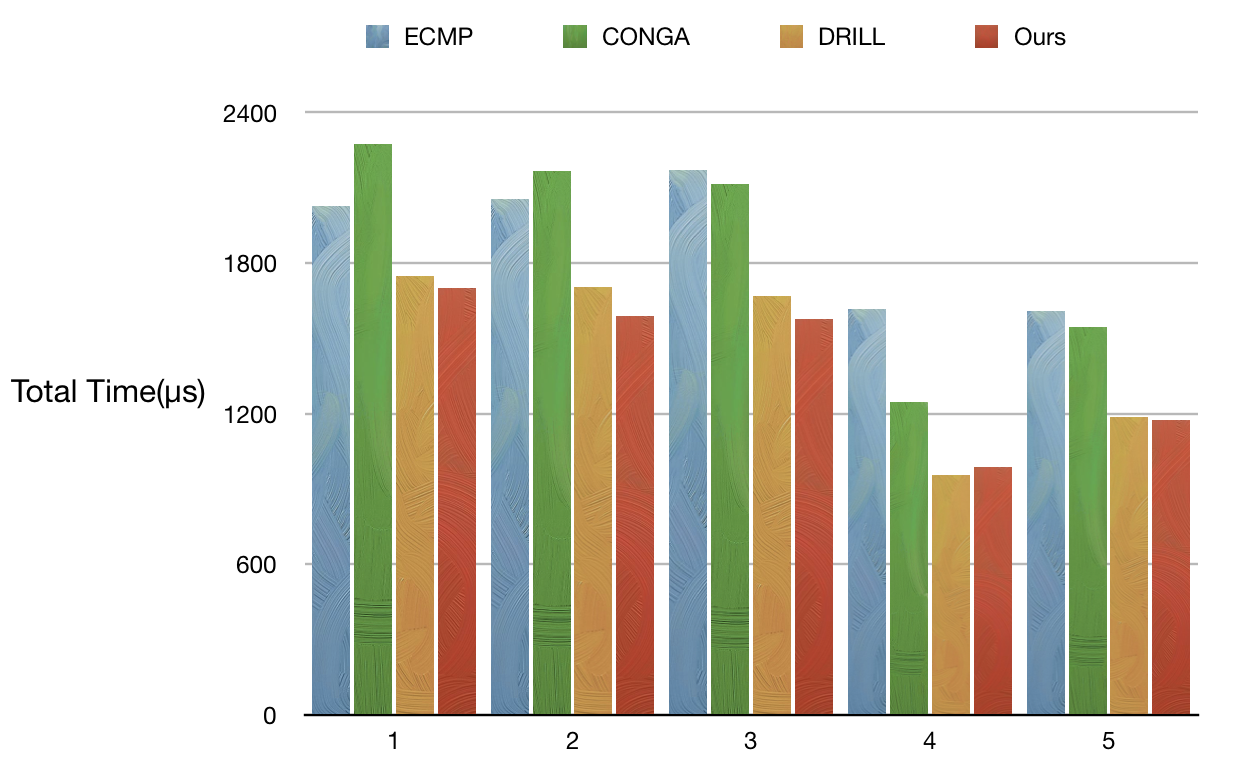
\includegraphics[height=5cm]{figure/total_time.png}
\caption{不同发送端的总传输时延}
\label{fig:total_time}
\end{figure}


\subsubsection{平均链路利用率}

如图\ref{fig:upleafagg}(a),可以看出在上行链路叶结点交换机的端口利用率上,CONGA在一开始的利用率要高于另外两种算法,这是因为初始时端口的拥塞并不严重,可以根据不同端口的拥塞情况来选择端口,因此利用率更高。后一时刻的利用率下降是因为这个周期的数据包已经传输完毕。本文提出的流量优化系统的端口利用率在特定情况下较高,这是因为对于长数据流而言,其流速率、转发路径、优先级由中心组件的离散增强学习算法单独确定,会导致其利用与普通数据流不同的端口。聚合交换机的端口利用率情况与叶结点交换机类似,这是因为叶结点交换机选择的两个端口对应两个聚合交换机,而每个聚合交换机仅有一个端口通向核心交换机,因此数据量与利用率情况类似(由图\ref{fig:netw_archi}的拓扑结构决定)。

\begin{figure*}[htb!]
\centering
\begin{subfigure}{0.47\textwidth}
     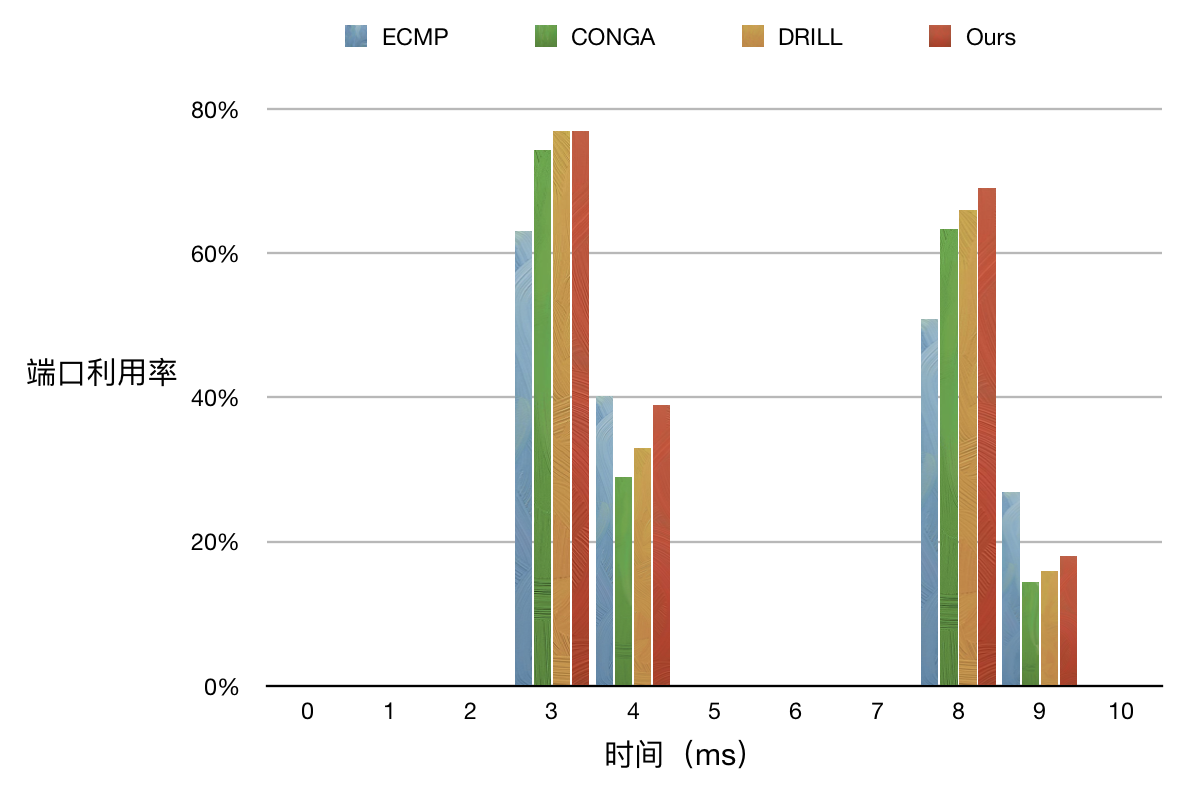
\includegraphics[width=\textwidth]{figure/upleaf.png}
     \caption{上行链路叶结点交换机的端口利用率}
\end{subfigure}\hspace{2em}
\begin{subfigure}{0.47\textwidth}
%\centering
    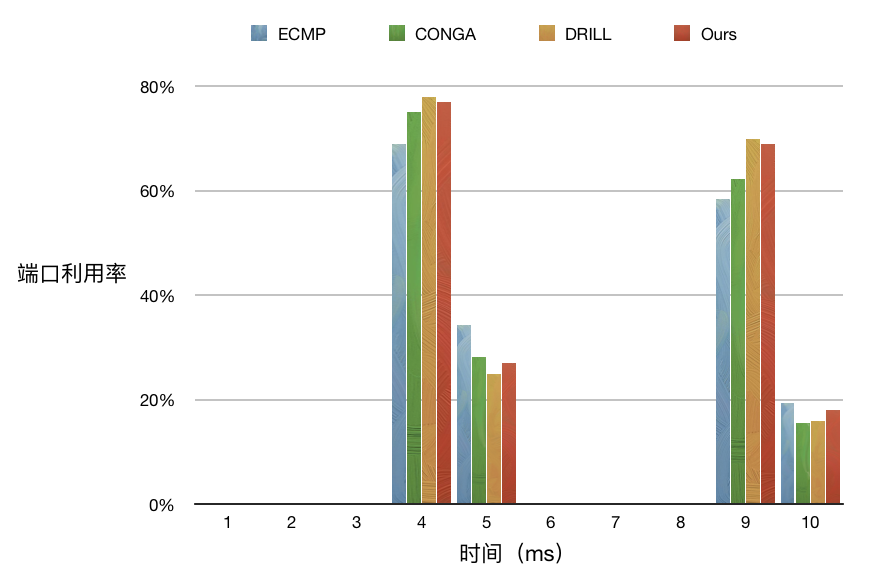
\includegraphics[width=\textwidth]{figure/upagg.png}
    \caption{上行链路聚合交换机的端口利用率}

\end{subfigure}%\hspace{0.277em}
\caption{上行平均链路利用率}
\label{fig:upleafagg}
\end{figure*}


对于下行链路(如图\ref{fig:downcoreagg}),四种算法在端口上的平均利用率基本相同,这是因为在核心交换机上均采用了ECMP,所以端口利用情况基本相同(DRILL主要针对Clos网络的二层结构,对于具有核心交换机的场景没有特殊处理)。


\begin{figure*}[htb!]
\centering
\begin{subfigure}{0.47\textwidth}
     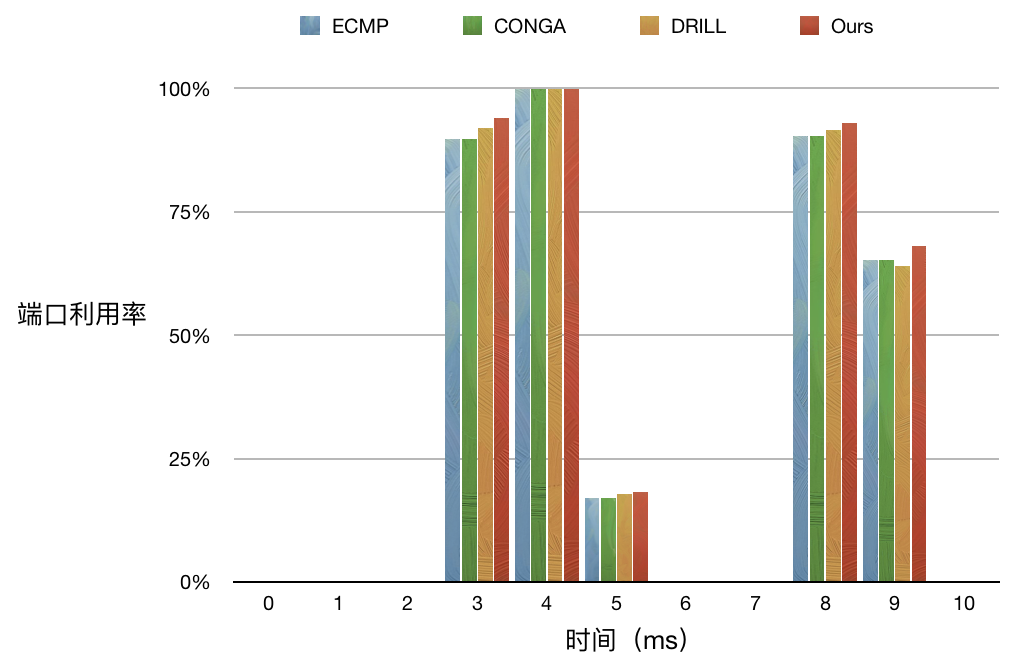
\includegraphics[width=\textwidth]{figure/downcore.png}
     \caption{下行链路核心交换机的端口利用率}
\end{subfigure}\hspace{2em}
\begin{subfigure}{0.47\textwidth}
%\centering
    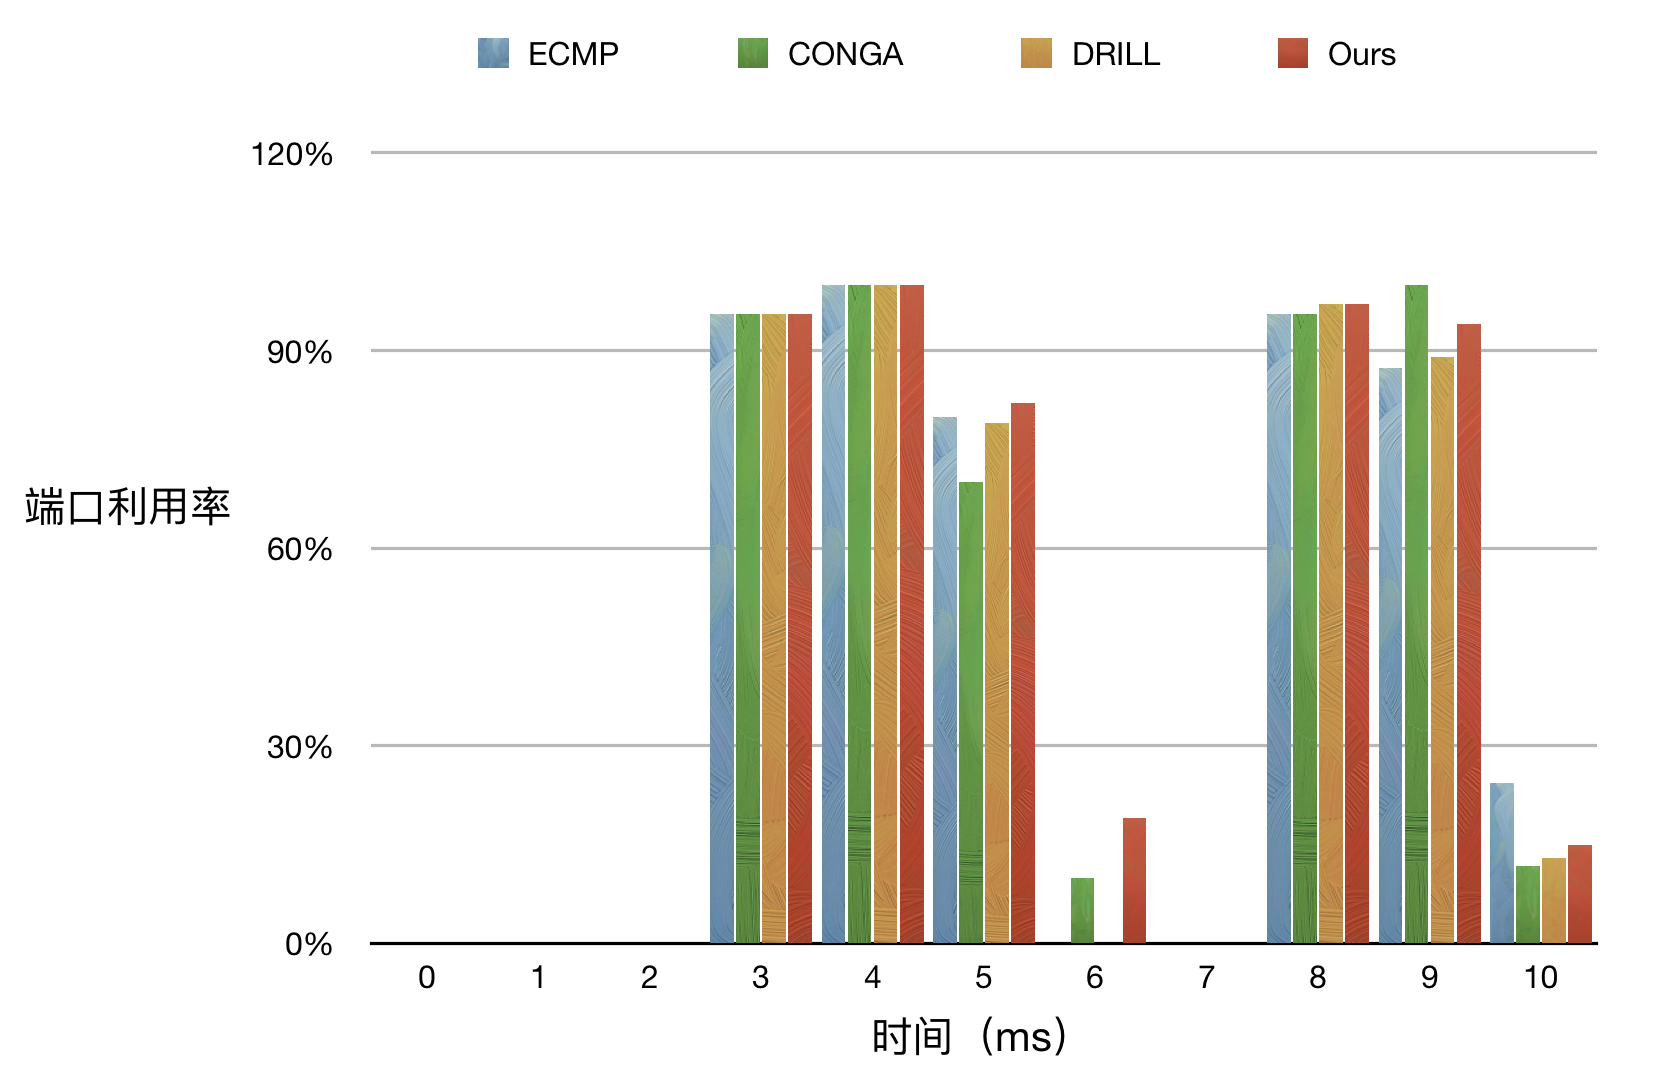
\includegraphics[width=\textwidth]{figure/downagg.png}
    \caption{下行链路聚合交换机的端口利用率}

\end{subfigure}%\hspace{0.277em}
\caption{下行平均链路利用率}
\label{fig:downcoreagg}
\end{figure*}



\subsection{性能分析}
可以看出,通过将DRILL负载均衡机制与流量调度算法相结合,对长数据流和短数据流分开处理,可以实时动态地控制数据传输选择最合适的路径,缩短数据流的完成时间,减少总传输时间,在特定情况中提升链路利用率以实现数据中心网络中的流量优化。当然,本文提出的架构也有需要改进的地方:与CONGA算法相似,DRILL负载均衡机制在三层网络中的性能有待加强,在核心交换机出只靠ECMP算法可能导致较大的问题;当整个链路的数据量较大时,基于本地的拥塞信息很容易判断为达到最大值,此时只能根据算法随机选择,因此拥塞情况可能不会以最快速度消失。

综上所述,本文提出对流量优化系统能够实现良好的负载均衡效果,能有效降低数据流的完成时间,增加链路利用率,对拥塞问题可以得到很好的解决,从性能上看,由于加入了PIAS架构中的MLFQ优先级队列,并利用近年来提出的深度增强学习算法,使得系统性能对于现有的负载均衡算法有较明显的提升。

